% ==========================================================================
% INFO 4617 Web Data Science -- Week 8: Dynamic Web Pages with Selenium (Chapter 8)
% Build:  latexmk -pdf week-08.tex   (from this folder; no env vars needed)
% (or run `make` from the slides/ directory to build every deck)
% ==========================================================================
\documentclass[9pt,aspectratio=169]{beamer}
% Resolve the shared theme/preamble in ../common/ when compiling this
% file directly from its own folder (no TEXINPUTS needed).
\makeatletter\def\input@path{{../common/}}\makeatother
% ==========================================================================
% Shared preamble for INFO 4617 Web Data Science weekly lecture decks
% Based on the Gotham beamer theme (vendored in this directory).
% Each week's slides.tex does:  % ==========================================================================
% Shared preamble for INFO 4617 Web Data Science weekly lecture decks
% Based on the Gotham beamer theme (vendored in this directory).
% Each week's slides.tex does:  % ==========================================================================
% Shared preamble for INFO 4617 Web Data Science weekly lecture decks
% Based on the Gotham beamer theme (vendored in this directory).
% Each week's slides.tex does:  \input{preamble}  (with common/ on TEXINPUTS)
% then sets \title/\subtitle/\author/\date and \begin{document}.
% ==========================================================================

\usetheme{gotham}

\usepackage{fbb}
\usepackage{booktabs}
\usepackage{graphicx}
\usepackage{tikz}
\usepackage{xcolor}
\usepackage{multirow}
\usepackage{listings}
\usetikzlibrary{positioning, arrows.meta, shapes}

% Bibliography
\usepackage[style=authoryear,
            backend=biber,
            maxcitenames=1,
            uniquename=false,
            uniquelist=false]{biblatex}
\addbibresource{bibliography.bib}

\gothamset{sectiontocframe default=off}

% ------------------------------------------------------------------ colors
\definecolor{cugold}{HTML}{CFB87C}
\definecolor{tab-red}{HTML}{E15759}
\definecolor{tab-orange}{HTML}{F28E2B}
\definecolor{tab-blue}{HTML}{4E79A7}
\definecolor{tab-cyan}{HTML}{76B7B2}
\definecolor{tab-green}{HTML}{59A14F}
\definecolor{tab-yellow}{HTML}{EDC948}
\definecolor{tab-purple}{HTML}{B07AA1}
\definecolor{tab-pink}{HTML}{FF9DA7}
\definecolor{tab-brown}{HTML}{9C755F}
\definecolor{tab-gray}{HTML}{BAB0AC}

\setbeamercolor{frametitle}{fg=black, bg=cugold}
\setbeamercolor{progress bar}{fg=cugold, bg=cugold!20}

\setbeamercolor{block title alerted}{fg=black, bg=cugold}
\setbeamercolor{block body alerted}{fg=black, bg=cugold!10}

% ------------------------------------------------------------------ footline
\setbeamertemplate{footline}{
  \begin{beamercolorbox}[wd=\paperwidth,ht=2.5ex,dp=1ex,right]{footline}
    {\footnotesize \insertframenumber{} of \inserttotalframenumber}
    \hspace*{2ex}
  \end{beamercolorbox}
}

% ------------------------------------------------------------------ helpers
\newcommand{\bottomcite}[1]{
    \vspace*{\fill}
    \vspace{-\baselineskip}
    {\tiny
    \rule{\textwidth}{0.3pt}\\
    #1
    }
    \vspace{0.5ex}
}

% Consistent code styling for the Wednesday "applied notebook" frames.
\lstdefinestyle{wds}{
    basicstyle=\ttfamily\scriptsize,
    keywordstyle=\color{tab-blue}\bfseries,
    commentstyle=\color{tab-green},
    stringstyle=\color{tab-orange},
    showstringspaces=false,
    breaklines=true,
    columns=fullflexible,
    language=Python,
    aboveskip=0.4em,
    belowskip=0.4em,
}
\lstset{style=wds}

% \dayband{Day}{Topic} -- a lightweight section divider label used to mark
% Monday / Wednesday / Friday within a week's deck.
\newcommand{\dayband}[2]{{\large\textbf{#1}}\;\textcolor{tab-gray}{\textbar}\;#2}
  (with common/ on TEXINPUTS)
% then sets \title/\subtitle/\author/\date and \begin{document}.
% ==========================================================================

\usetheme{gotham}

\usepackage{fbb}
\usepackage{booktabs}
\usepackage{graphicx}
\usepackage{tikz}
\usepackage{xcolor}
\usepackage{multirow}
\usepackage{listings}
\usetikzlibrary{positioning, arrows.meta, shapes}

% Bibliography
\usepackage[style=authoryear,
            backend=biber,
            maxcitenames=1,
            uniquename=false,
            uniquelist=false]{biblatex}
\addbibresource{bibliography.bib}

\gothamset{sectiontocframe default=off}

% ------------------------------------------------------------------ colors
\definecolor{cugold}{HTML}{CFB87C}
\definecolor{tab-red}{HTML}{E15759}
\definecolor{tab-orange}{HTML}{F28E2B}
\definecolor{tab-blue}{HTML}{4E79A7}
\definecolor{tab-cyan}{HTML}{76B7B2}
\definecolor{tab-green}{HTML}{59A14F}
\definecolor{tab-yellow}{HTML}{EDC948}
\definecolor{tab-purple}{HTML}{B07AA1}
\definecolor{tab-pink}{HTML}{FF9DA7}
\definecolor{tab-brown}{HTML}{9C755F}
\definecolor{tab-gray}{HTML}{BAB0AC}

\setbeamercolor{frametitle}{fg=black, bg=cugold}
\setbeamercolor{progress bar}{fg=cugold, bg=cugold!20}

\setbeamercolor{block title alerted}{fg=black, bg=cugold}
\setbeamercolor{block body alerted}{fg=black, bg=cugold!10}

% ------------------------------------------------------------------ footline
\setbeamertemplate{footline}{
  \begin{beamercolorbox}[wd=\paperwidth,ht=2.5ex,dp=1ex,right]{footline}
    {\footnotesize \insertframenumber{} of \inserttotalframenumber}
    \hspace*{2ex}
  \end{beamercolorbox}
}

% ------------------------------------------------------------------ helpers
\newcommand{\bottomcite}[1]{
    \vspace*{\fill}
    \vspace{-\baselineskip}
    {\tiny
    \rule{\textwidth}{0.3pt}\\
    #1
    }
    \vspace{0.5ex}
}

% Consistent code styling for the Wednesday "applied notebook" frames.
\lstdefinestyle{wds}{
    basicstyle=\ttfamily\scriptsize,
    keywordstyle=\color{tab-blue}\bfseries,
    commentstyle=\color{tab-green},
    stringstyle=\color{tab-orange},
    showstringspaces=false,
    breaklines=true,
    columns=fullflexible,
    language=Python,
    aboveskip=0.4em,
    belowskip=0.4em,
}
\lstset{style=wds}

% \dayband{Day}{Topic} -- a lightweight section divider label used to mark
% Monday / Wednesday / Friday within a week's deck.
\newcommand{\dayband}[2]{{\large\textbf{#1}}\;\textcolor{tab-gray}{\textbar}\;#2}
  (with common/ on TEXINPUTS)
% then sets \title/\subtitle/\author/\date and \begin{document}.
% ==========================================================================

\usetheme{gotham}

\usepackage{fbb}
\usepackage{booktabs}
\usepackage{graphicx}
\usepackage{tikz}
\usepackage{xcolor}
\usepackage{multirow}
\usepackage{listings}
\usetikzlibrary{positioning, arrows.meta, shapes}

% Bibliography
\usepackage[style=authoryear,
            backend=biber,
            maxcitenames=1,
            uniquename=false,
            uniquelist=false]{biblatex}
\addbibresource{bibliography.bib}

\gothamset{sectiontocframe default=off}

% ------------------------------------------------------------------ colors
\definecolor{cugold}{HTML}{CFB87C}
\definecolor{tab-red}{HTML}{E15759}
\definecolor{tab-orange}{HTML}{F28E2B}
\definecolor{tab-blue}{HTML}{4E79A7}
\definecolor{tab-cyan}{HTML}{76B7B2}
\definecolor{tab-green}{HTML}{59A14F}
\definecolor{tab-yellow}{HTML}{EDC948}
\definecolor{tab-purple}{HTML}{B07AA1}
\definecolor{tab-pink}{HTML}{FF9DA7}
\definecolor{tab-brown}{HTML}{9C755F}
\definecolor{tab-gray}{HTML}{BAB0AC}

\setbeamercolor{frametitle}{fg=black, bg=cugold}
\setbeamercolor{progress bar}{fg=cugold, bg=cugold!20}

\setbeamercolor{block title alerted}{fg=black, bg=cugold}
\setbeamercolor{block body alerted}{fg=black, bg=cugold!10}

% ------------------------------------------------------------------ footline
\setbeamertemplate{footline}{
  \begin{beamercolorbox}[wd=\paperwidth,ht=2.5ex,dp=1ex,right]{footline}
    {\footnotesize \insertframenumber{} of \inserttotalframenumber}
    \hspace*{2ex}
  \end{beamercolorbox}
}

% ------------------------------------------------------------------ helpers
\newcommand{\bottomcite}[1]{
    \vspace*{\fill}
    \vspace{-\baselineskip}
    {\tiny
    \rule{\textwidth}{0.3pt}\\
    #1
    }
    \vspace{0.5ex}
}

% Consistent code styling for the Wednesday "applied notebook" frames.
\lstdefinestyle{wds}{
    basicstyle=\ttfamily\scriptsize,
    keywordstyle=\color{tab-blue}\bfseries,
    commentstyle=\color{tab-green},
    stringstyle=\color{tab-orange},
    showstringspaces=false,
    breaklines=true,
    columns=fullflexible,
    language=Python,
    aboveskip=0.4em,
    belowskip=0.4em,
}
\lstset{style=wds}

% \dayband{Day}{Topic} -- a lightweight section divider label used to mark
% Monday / Wednesday / Friday within a week's deck.
\newcommand{\dayband}[2]{{\large\textbf{#1}}\;\textcolor{tab-gray}{\textbar}\;#2}


\title[Week 8 · Dynamic Pages]{{\Huge Dynamic Web Pages with Selenium}}
\subtitle{Week 8 · Documents module · Textbook Chapter 8}
\author[Keegan]{\textbf{Brian C. Keegan, Ph.D.} \\ Associate Professor, Department of Information Science \\ University of Colorado Boulder}
\date{October 5, 7 \& 9, 2026}

\begin{document}

\maketitle

% -------------------------------------------------------------------------
\begin{frame}{This week at a glance}
    \begin{columns}[T]
        \begin{column}{0.6\textwidth}
            Most of the modern web renders its data with JavaScript \textit{after} the HTML arrives. This week: check whether you need a browser, then drive one.

            \bigskip

            \dayband{Monday}{Concepts \& notebook intro}
            \begin{itemize}\small
                \item Three checks by hand; Selenium and Selenium Manager; Playwright scripts; AI agents that drive a browser
                \item Close with a pair activity: do you need a browser?
            \end{itemize}

            \medskip

            \dayband{Wednesday}{Notebook lab}
            \begin{itemize}\small
                \item Work the Chapter 8 notebook in Selenium: xkcd, a Wikipedia search, and the Quotes to Scrape sandbox
            \end{itemize}

            \medskip

            \dayband{Friday}{Textbook revisions}
            \begin{itemize}\small
                \item Propose \& peer-review pull requests improving Chapter 8
            \end{itemize}
        \end{column}
        \begin{column}{0.35\textwidth}
            \begin{block}{Companion notebook}
                \footnotesize \texttt{ch-08-dynamic-pages.ipynb}
            \end{block}
            \begin{alertblock}{Bring a laptop}
                \footnotesize Monday and Wednesday are both hands-on --- bring a laptop both days.
            \end{alertblock}
        \end{column}
    \end{columns}
\end{frame}

% =========================================================================
\section{Monday · Concepts}
% =========================================================================

\begin{frame}{Zero bytes}
    \begin{center}
        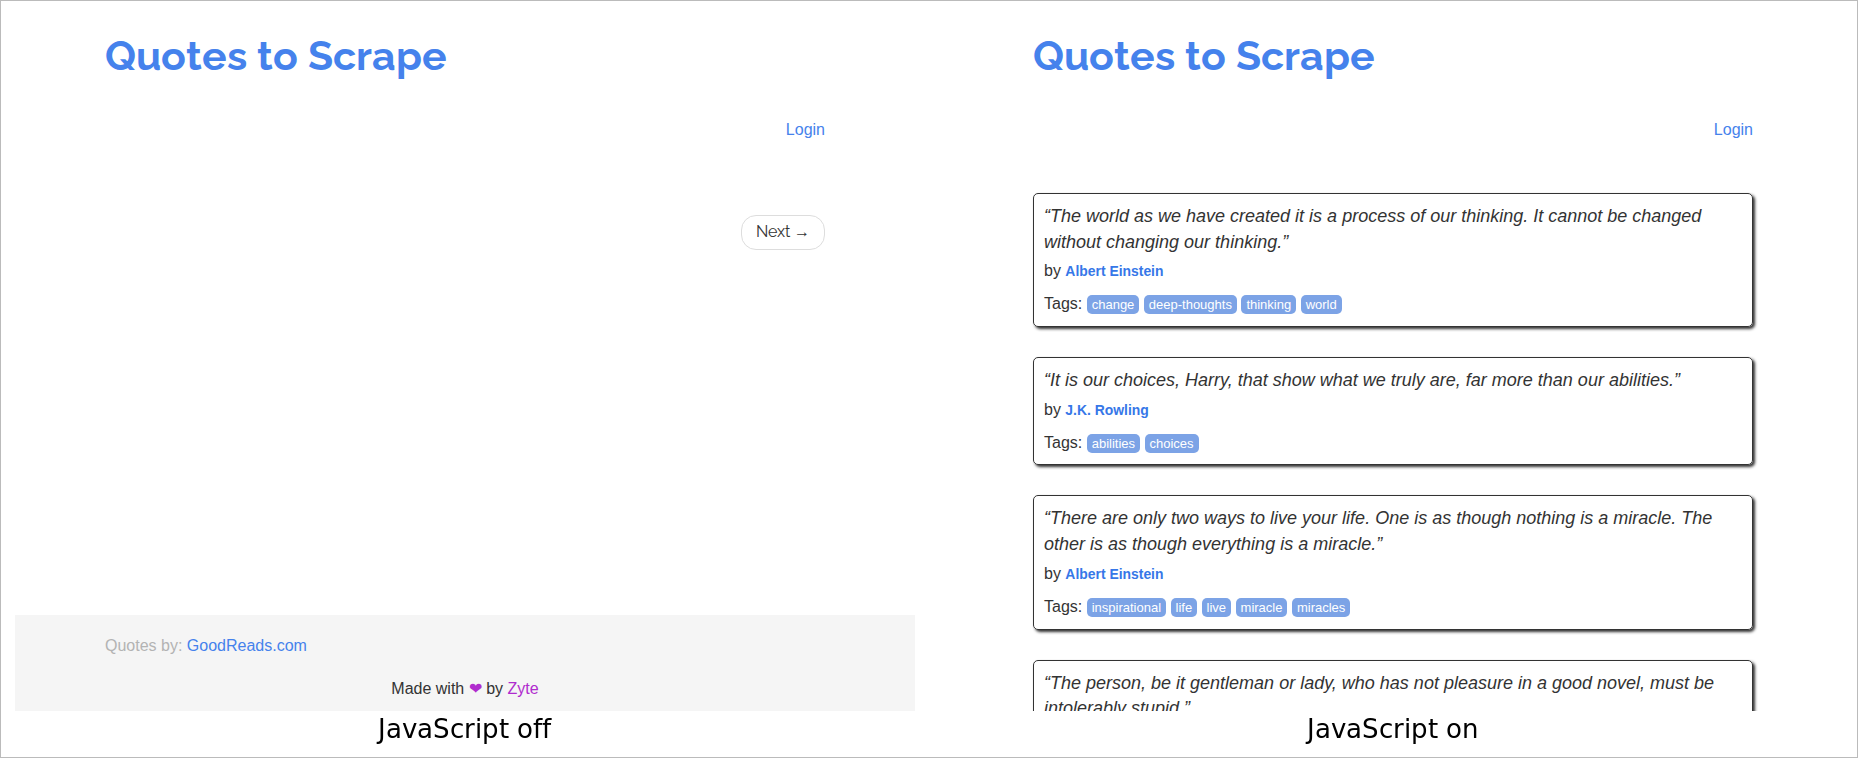
\includegraphics[width=0.78\textwidth]{img/requests_vs_browser.png}\\
        {\scriptsize Same URL, two very different pages: \texttt{quotes.toscrape.com/js/}, JavaScript off and on.}
    \end{center}

    Week~6 ended here: IMDb answered \texttt{requests.get()} with status 202 and zero bytes of HTML. A browser showed the whole page.

    \medskip
    Most modern sites are \textbf{dynamic}. JavaScript builds the content \textit{after} the HTML arrives, and \texttt{requests} never runs JavaScript.
\end{frame}

\begin{frame}{Check by hand first}
    \begin{columns}[T]
        \begin{column}{0.45\textwidth}
            Driving a browser is slow and fragile. Three checks in your own browser settle most pages, about a minute each.

            \bigskip
            \textbf{View Source.} Is the data in what the server sent?

            \medskip
            \textbf{JavaScript off.} What is left without it?

            \medskip
            \textbf{Network tab.} Does the data arrive as JSON?

            \bigskip
            The examples use Quotes to Scrape, a sandbox built for scraping practice.
        \end{column}
        \begin{column}{0.52\textwidth}
            \centering
            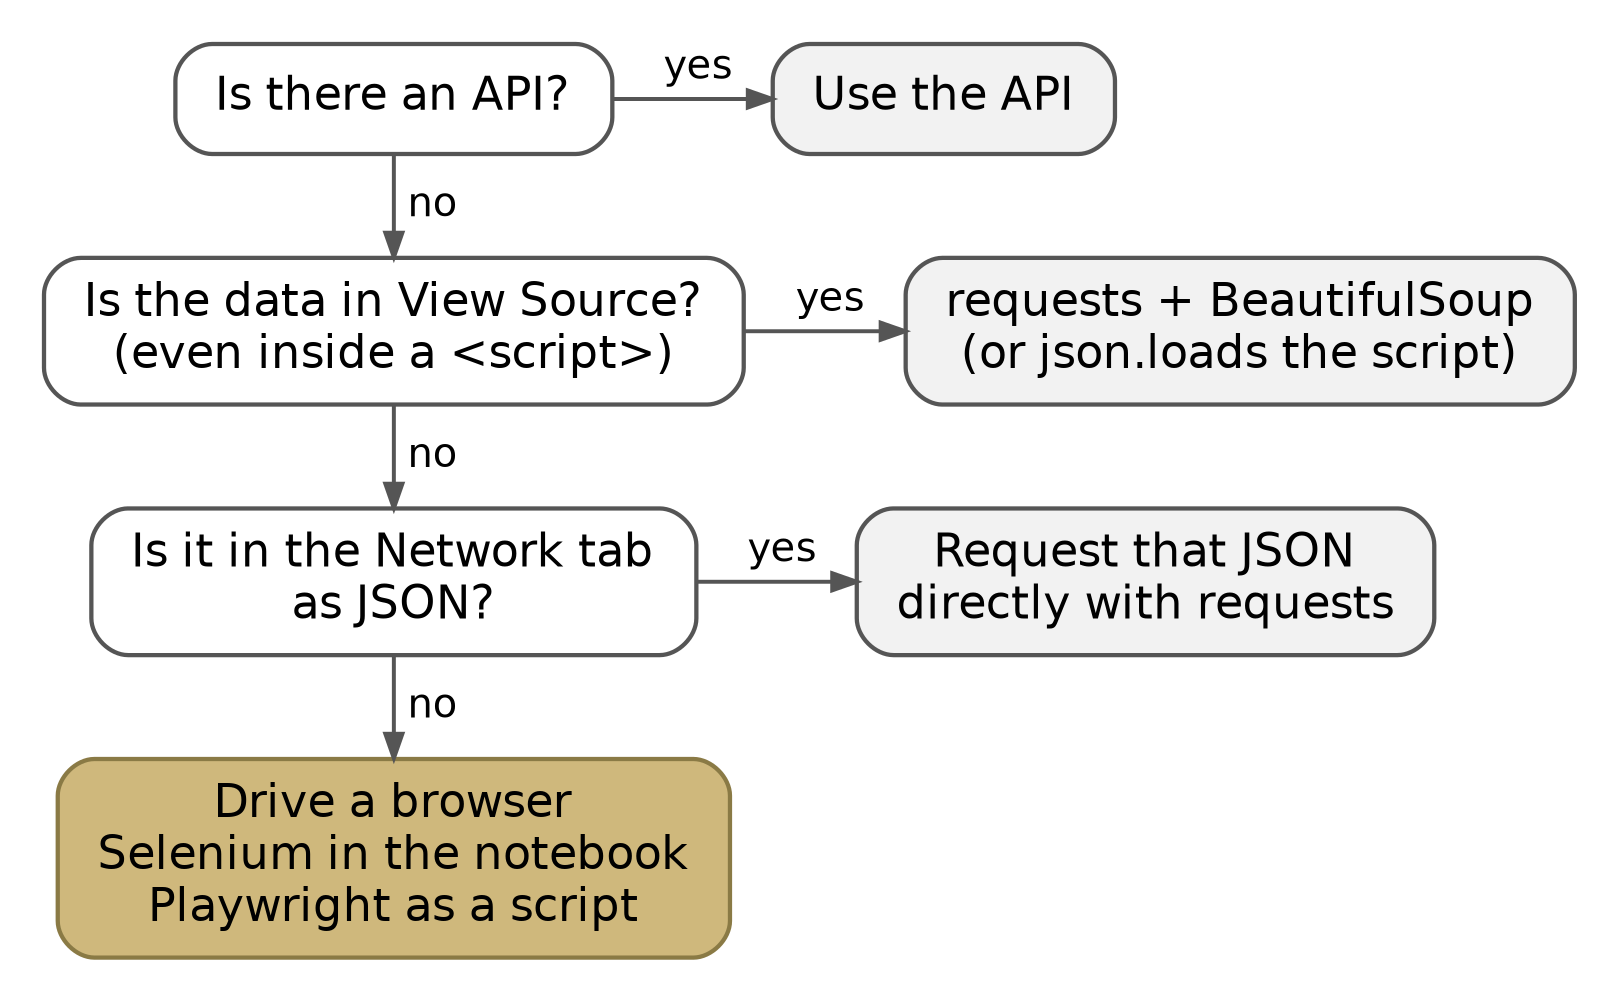
\includegraphics[width=\textwidth]{img/decision_tree.png}
        \end{column}
    \end{columns}
\end{frame}

\begin{frame}{Check 1: View Source}
    \begin{center}
        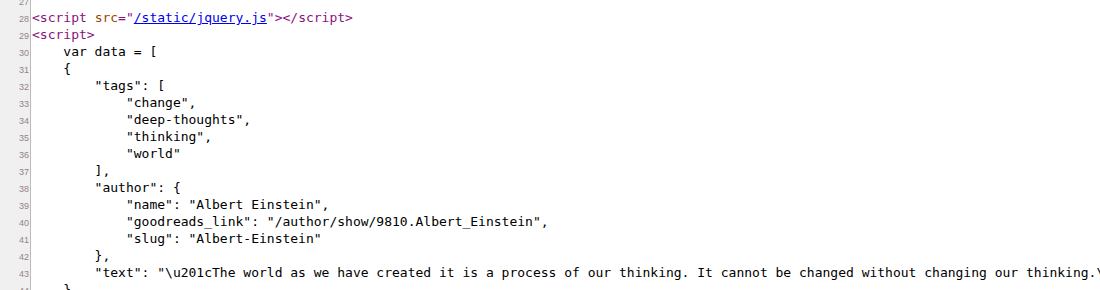
\includegraphics[width=0.92\textwidth]{img/view_source_js.png}
    \end{center}

    \texttt{requests} finds zero \texttt{div.quote} elements on \texttt{quotes.toscrape.com/js/}. View Source shows why: there is no quote markup at all.

    \medskip
    But the quotes are in the file --- inside a \texttt{<script>}, as a JavaScript array. \texttt{re.search()} cuts it out and \texttt{json.loads()} parses it. Ten quotes, no browser.
\end{frame}

\begin{frame}{Check 2: JavaScript off}
    \begin{columns}[T]
        \begin{column}{0.6\textwidth}
            Open DevTools. Press Ctrl+Shift+P (Cmd+Shift+P on a Mac). Type \texttt{javascript}. Choose \textbf{Disable JavaScript}. Reload the page.

            \bigskip
            What is left is roughly what \texttt{requests} gets: a title, a login link, a Next button. No quotes.

            \bigskip
            JavaScript stays off only while DevTools is open.
        \end{column}
        \begin{column}{0.35\textwidth}
            \centering
            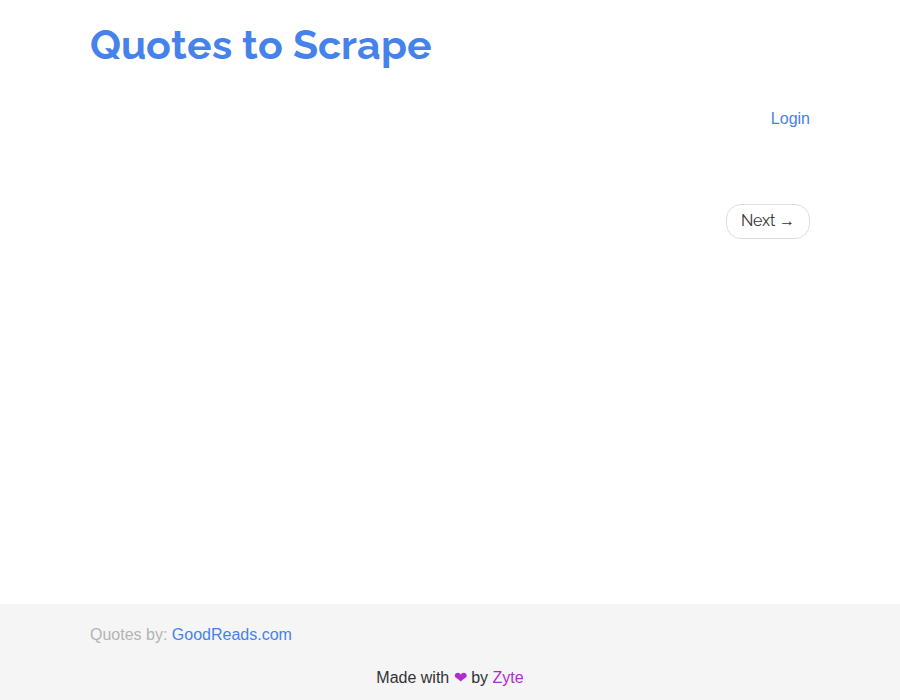
\includegraphics[width=\textwidth]{img/js_off.png}\\
            {\scriptsize The same page, JavaScript off.}
        \end{column}
    \end{columns}
\end{frame}

\begin{frame}{Check 3: the Network tab}
    \begin{center}
        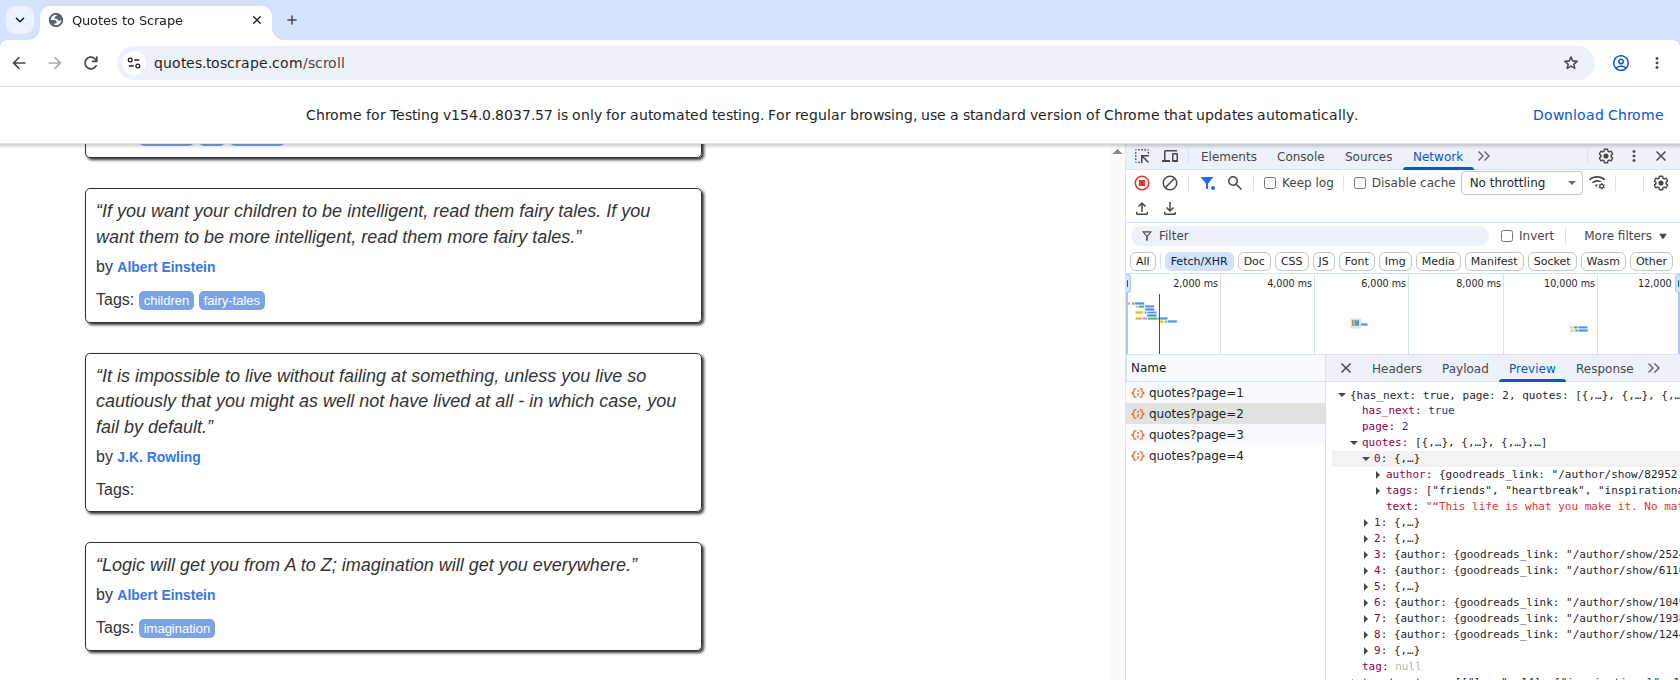
\includegraphics[width=0.8\textwidth]{img/network_json.png}
    \end{center}

    On \texttt{quotes.toscrape.com/scroll}, filter the Network tab to \textbf{Fetch/XHR} and scroll. Each page of quotes arrives as JSON from \texttt{/api/quotes?page=N}.

    \medskip
    Request that JSON yourself: 100 quotes over 10 pages, with \texttt{requests} and a one-second pause between pages. No browser.
\end{frame}

\begin{frame}{Selenium: a browser you drive with code}
    \begin{columns}[T]
        \begin{column}{0.6\textwidth}
            When all three checks come up empty, you need a real browser.

            \bigskip
            \texttt{pip install selenium}, then \texttt{driver = webdriver.Chrome()} opens a window. Every command you give \texttt{driver} happens in that window.

            \bigskip
            You are not faking HTTP requests anymore. You are \textbf{automating a browser}, the same one a person would use.
        \end{column}
        \begin{column}{0.35\textwidth}
            \centering
            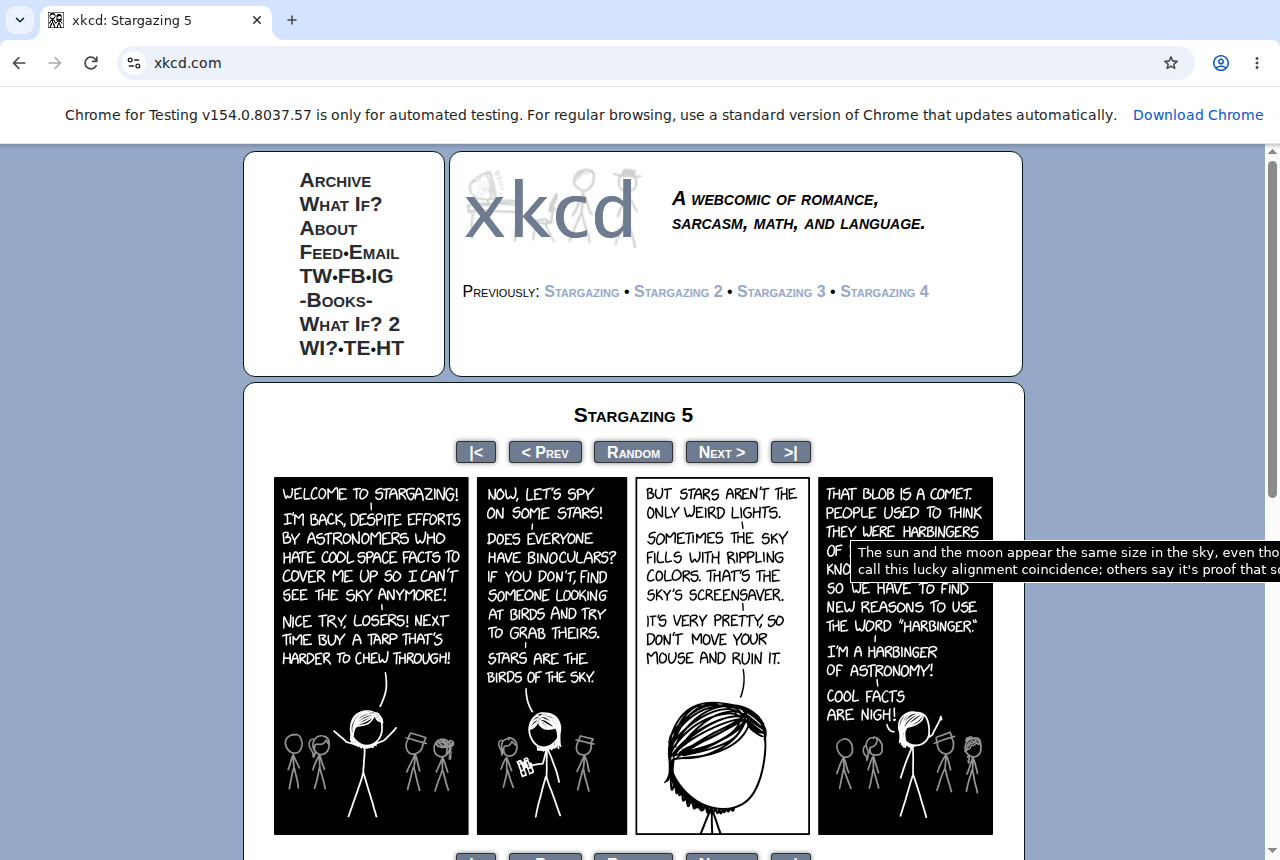
\includegraphics[width=\textwidth]{img/selenium_browser.png}\\
            {\scriptsize Chrome for Testing, driven by Selenium.}
        \end{column}
    \end{columns}
\end{frame}

\begin{frame}[fragile]{Selenium Manager}
    \begin{columns}[T]
        \begin{column}{0.6\textwidth}
            A small program inside the \texttt{selenium} package. \texttt{webdriver.Chrome()} runs it first.

            \medskip
            It finds your Chrome, or downloads Chrome for Testing if you have none. It finds the matching driver, downloads it, and caches both in \texttt{\textasciitilde/.cache/selenium}.

            \medskip
            It also sends anonymous usage statistics, unless you set \texttt{SE\_AVOID\_STATS=true}.
        \end{column}
        \begin{column}{0.35\textwidth}
            \centering
            
\includegraphics[width=0.8\textwidth]{img/meme_it_just_works.png}
        \end{column}
    \end{columns}
\begin{lstlisting}
chrome not found in the system
Required browser: chrome 154.0.8037.57
Downloading chrome 154.0.8037.57 from https://storage.googleapis.com/...
Required driver: chromedriver 154.0.8037.57
\end{lstlisting}
\end{frame}

\begin{frame}[fragile]{When it doesn't}
    An old \texttt{chromedriver} on your \texttt{PATH} beats the one Selenium Manager picks:
\begin{lstlisting}
Found chromedriver 147.0.7727.24 in PATH: /opt/node22/bin/chromedriver
Driver path: /opt/node22/bin/chromedriver
SessionNotCreatedException: session not created: This version of
ChromeDriver only supports Chrome version 147
Current browser version is 154.0.8037.57
\end{lstlisting}
    \begin{columns}[T]
        \begin{column}{0.6\textwidth}\small
            \textbf{Stray driver?} Delete it, or set \texttt{SE\_SKIP\_DRIVER\_IN\_PATH=true}

            \smallskip
            \textbf{Campus firewall?} Set \texttt{SE\_PROXY}, or run once off campus

            \smallskip
            \textbf{Browser from conda or snap?} Set \texttt{options.binary\_location}

            \smallskip
            \textbf{Stuck cache?} Delete \texttt{\textasciitilde/.cache/selenium}
        \end{column}
        \begin{column}{0.35\textwidth}
            \begin{alertblock}{Set it in Python}
                \footnotesize \texttt{os.environ["SE\_SKIP\_DRIVER\_IN\_PATH"] = "true"} before your first \texttt{webdriver.Chrome()}
            \end{alertblock}
        \end{column}
    \end{columns}
\end{frame}

\begin{frame}{Playwright}
    \begin{columns}[T]
        \begin{column}{0.6\textwidth}
            Microsoft, January 2020, built by engineers who had worked on Google's Puppeteer.

            \bigskip
            It brings its own browsers: \texttt{pip install playwright}, then \texttt{playwright install chromium}. About 300\,MB of downloads.

            \bigskip
            It waits for elements on its own, and it records a script while you click.

            \bigskip
            It runs best as a script from the terminal, not in a notebook.
        \end{column}
        \begin{column}{0.35\textwidth}
            \centering
            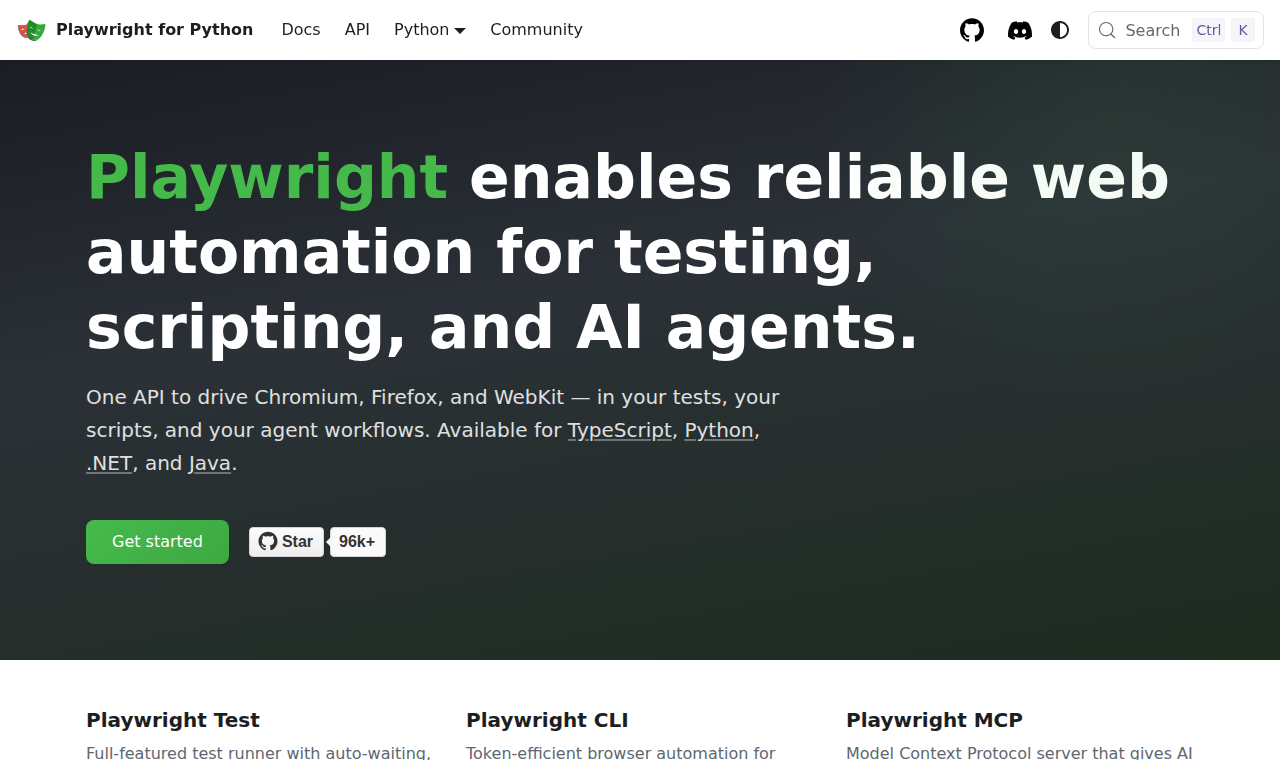
\includegraphics[width=\textwidth]{img/playwright_home.png}\\
            {\scriptsize playwright.dev/python, September 2026.}
        \end{column}
    \end{columns}
\end{frame}

\begin{frame}[fragile]{A Playwright script}
    Save it as \texttt{xkcd\_alt.py}. Run \texttt{python xkcd\_alt.py} in a terminal.
\begin{lstlisting}
from playwright.sync_api import sync_playwright

with sync_playwright() as p:
    browser = p.chromium.launch()      # headless by default
    page = browser.new_page()
    page.goto("https://xkcd.com")
    img = page.locator("#comic img")
    print(img.get_attribute("alt"))    # the comic's name
    print(img.get_attribute("title"))  # the hover joke
    browser.close()
\end{lstlisting}
    \texttt{page} plays \texttt{driver}. \texttt{page.goto()} plays \texttt{driver.get()}. A \textbf{locator} plays \texttt{find\_element()}. The \texttt{with} block is your \texttt{driver.quit()}.
\end{frame}

\begin{frame}[fragile]{Locators wait for you}
    This sandbox page waits ten seconds before its JavaScript adds the quotes:
\begin{lstlisting}
page.goto("https://quotes.toscrape.com/js-delayed/")

page.locator("div.quote").count()                        # 0 -- does not wait
page.locator("div.quote span.text").first.inner_text()   # waits ~10 s
page.locator("div.quote").count()                        # 10
\end{lstlisting}
    Acting on an element, or reading from it, waits up to 30 seconds. Reporting on the page as it stands right now does not.

    \medskip
    Selenium needs \texttt{WebDriverWait} for the same page. You will write it on Wednesday.
\end{frame}

\begin{frame}[fragile]{Why not in the notebook?}
    \begin{columns}[T]
        \begin{column}{0.6\textwidth}
            Run that script in a Jupyter cell:
\begin{lstlisting}
Error: It looks like you are using
Playwright Sync API inside the asyncio
loop. Please use the Async API instead.
\end{lstlisting}
            Jupyter already runs an event loop. Playwright's simple sync API needs one of its own.

            \medskip
            The async API works in a notebook, with \texttt{await} in front of nearly every call. Forget one, and you get a placeholder instead of a result.
        \end{column}
        \begin{column}{0.35\textwidth}
            \centering
            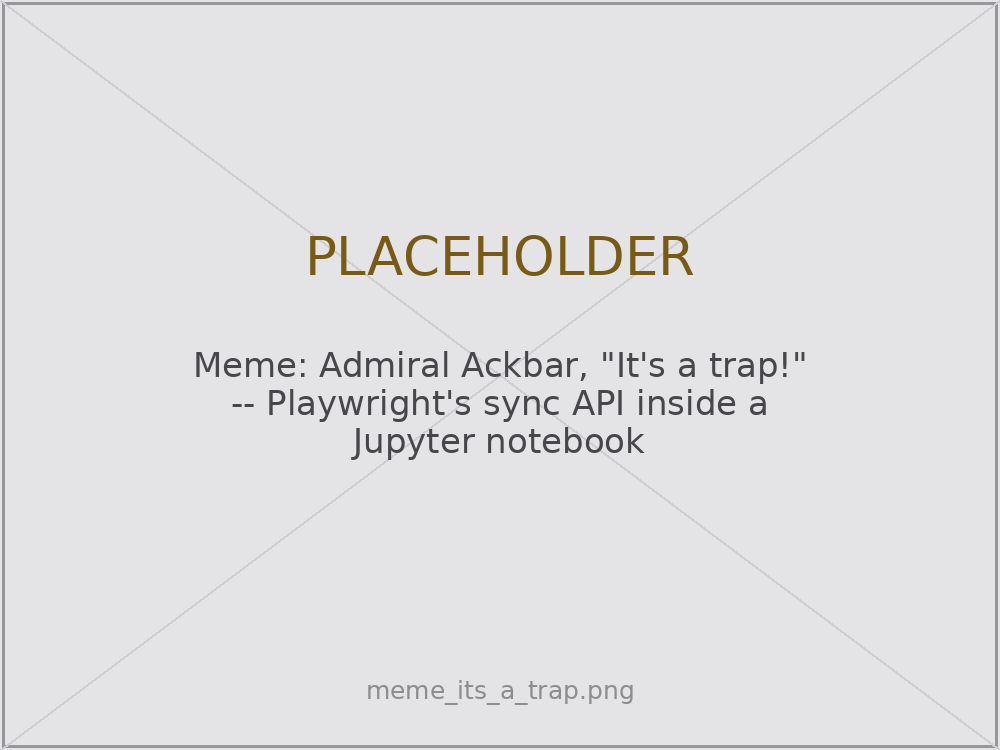
\includegraphics[width=\textwidth]{img/meme_its_a_trap.png}
        \end{column}
    \end{columns}
\end{frame}

\begin{frame}[fragile]{Record, then read}
    \begin{columns}[T]
        \begin{column}{0.42\textwidth}
            \texttt{playwright codegen https://quotes.toscrape.com/}

            \medskip
            Click in the browser. Each click becomes a line of Python:
\begin{lstlisting}
page.get_by_role("link",
    name="change").click()
page.get_by_role("link",
    name="(about)").click()
\end{lstlisting}
            Role-based locators survive a CSS redesign. They break when the visible text changes.

            \medskip
            A recording is a first draft. It clicks; it extracts nothing.
        \end{column}
        \begin{column}{0.55\textwidth}
            \centering
            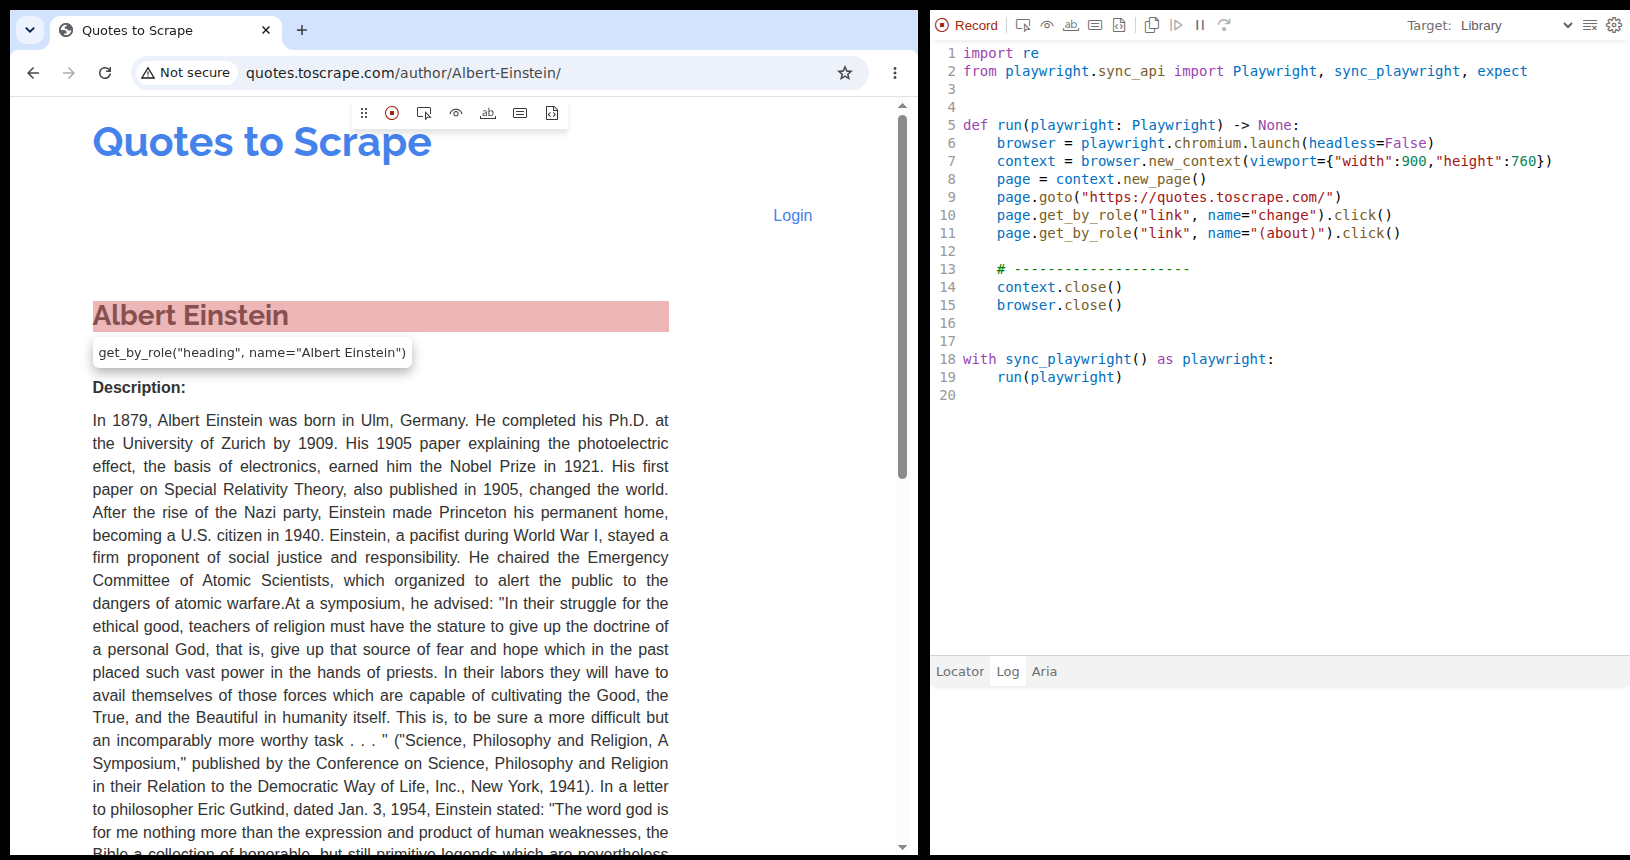
\includegraphics[width=\textwidth]{img/codegen.png}
        \end{column}
    \end{columns}
\end{frame}

\begin{frame}[fragile]{An assistant at the wheel}
    \begin{columns}[T]
        \begin{column}{0.6\textwidth}
            \textbf{MCP}, the Model Context Protocol, plugs outside tools into an AI assistant. \textbf{Playwright MCP} gives it a browser: \texttt{browser\_navigate}, \texttt{browser\_click}, \texttt{browser\_type}.

            \medskip
            These lines work in most MCP-capable assistants (Node.js 20 or newer):
\begin{lstlisting}
{ "mcpServers": {
    "playwright": {
      "command": "npx",
      "args": ["@playwright/mcp@latest"] } } }
\end{lstlisting}
            It opens a visible browser by default. Watch it.
        \end{column}
        \begin{column}{0.35\textwidth}
            \centering
            
\includegraphics[width=\textwidth]{img/meme_captain_now.png}
        \end{column}
    \end{columns}
\end{frame}

\begin{frame}[fragile]{What the agent sees}
    \begin{columns}[T]
        \begin{column}{0.5\textwidth}
            Not pixels. An \textbf{accessibility snapshot}: the page's parts by role and name, the same tree a screen reader uses.

            \bigskip
            Real links, labeled buttons, and \texttt{alt} text make a page easy for an agent. Unlabeled \texttt{<div>}s make it hard.

            \bigskip
            {\footnotesize xkcd, September 2026, from Playwright's \texttt{aria\_snapshot()}.}
        \end{column}
        \begin{column}{0.45\textwidth}
\begin{lstlisting}
- text: Stargazing 5
- list:
  - listitem:
    - link "|<":
      - /url: /1/
  - listitem:
    - link "< Prev":
      - /url: /3300/
  - listitem:
    - link "Random":
      - /url: //c.xkcd.com/random/comic/
  ...
- img "Stargazing 5"
\end{lstlisting}
        \end{column}
    \end{columns}
\end{frame}

\begin{frame}{Drive, or write the scraper?}
    \textbf{Let it drive.} ``Collect every quote tagged \textit{love} on quotes.toscrape.com.'' Flexible. But every run improvises, costs money, and can click something different.

    \bigskip
    \textbf{Let it write.} ``Write me a Playwright script that collects every quote tagged \textit{love}.'' You get code to read, test, commit, and rerun for free.

    \bigskip
    \textbf{Codegen.} No AI at all. Your own clicks become the script.

    \bigskip
    Which one could you describe in a methods section?
\end{frame}

\begin{frame}{An agent is still your scraper}
    \begin{columns}[T]
        \begin{column}{0.6\textwidth}
            Its requests are your requests. \texttt{robots.txt} and the Terms of Service still apply (Ch.~2).

            \medskip
            The page goes to the AI company along with your prompt. Keep agents away from private data.

            \medskip
            \textbf{Prompt injection:} text on a page, even text you cannot see, can give the agent new orders.

            \medskip
            Never let an agent drive a browser that is logged in to your accounts. It acts as you.
        \end{column}
        \begin{column}{0.35\textwidth}
            \begin{alertblock}{Automation is not a loophole}
                \footnotesize A \texttt{robots.txt} rule and a site's ToS still apply when a real browser --- or an AI --- does the clicking.
            \end{alertblock}

            \medskip
            {\scriptsize Not legal advice.}
        \end{column}
    \end{columns}
\end{frame}

\begin{frame}{Selenium or Playwright?}
    \centering\small
    \begin{tabular}{p{0.15\textwidth}p{0.37\textwidth}p{0.37\textwidth}}
        & \textbf{Selenium} & \textbf{Playwright} \tabularnewline \hline
        \raggedright Install & \raggedright \texttt{pip install selenium} & \raggedright \texttt{pip install playwright}, then \texttt{playwright install} \tabularnewline[0.5em]
        \raggedright Browsers & \raggedright Yours; Selenium Manager downloads Chrome for Testing if you have none & \raggedright Its own copies, pinned to each release \tabularnewline[0.5em]
        \raggedright Notebook & \raggedright Yes & \raggedright Only with the async API and \texttt{await} \tabularnewline[0.5em]
        \raggedright Waiting & \raggedright Explicit: \texttt{WebDriverWait} & \raggedright Automatic when you act on or read an element \tabularnewline[0.5em]
        \raggedright Recording & \raggedright Selenium IDE, a browser extension & \raggedright \texttt{playwright codegen}, built in \tabularnewline
    \end{tabular}

    \bigskip
    This course's lab and take-home use Selenium.
\end{frame}

\begin{frame}{Closing activity: do you need a browser?}
    \begin{columns}[T]
        \begin{column}{0.6\textwidth}\small
            Work in pairs. Pick a page that shows data you would want: a news live blog, a sports scoreboard, a store's search results, a campus events calendar.
            \begin{enumerate}
                \item Open View Source. Search it for a word you can see on the page
                \item Turn JavaScript off. Reload. Write down what is left
                \item Open the Network tab. Filter to Fetch/XHR. Reload, scroll, or click. Find the request that carries the data
                \item Decide: \texttt{requests}, the JSON directly, or a browser?
            \end{enumerate}

            \bigskip
            Stuck? Start with quotes.toscrape.com/js/ and quotes.toscrape.com/scroll

            \bigskip
            Report back with one page that did not need a browser, and one that did
        \end{column}
        \begin{column}{0.35\textwidth}
            \centering
            
\includegraphics[width=\textwidth]{img/meme_is_this_dynamic.png}
        \end{column}
    \end{columns}
\end{frame}

\begin{frame}{Before Wednesday}
    \begin{columns}[T]
        \begin{column}{0.6\textwidth}
            Complete daily note: \url{https://bit.ly/info4617f26}

            \medskip
            Read Textbook Ch.~8 before Wednesday.

            \medskip
            Install Selenium before class: \texttt{pip install selenium}. Your first \texttt{webdriver.Chrome()} may download a driver, and Chrome too if you have none. Do it on a fast connection.
        \end{column}
        \begin{column}{0.35\textwidth}
            \begin{alertblock}{Wednesday lab}
                \small Complete \textbf{Recommended Exercises}: fill in the empty cells, run everything, export to HTML, upload to Canvas by \textbf{Sunday 11:59pm}
            \end{alertblock}
            \begin{alertblock}{Friday}
                \small Upload the link to your pull request or issue by \textbf{Sunday 11:59pm}
            \end{alertblock}
        \end{column}
    \end{columns}
\end{frame}

% =========================================================================
\section{Wednesday · Notebook Lab}
% =========================================================================

\begin{frame}[fragile]{Launch a driver, then locate elements}
    Four strategies find elements; \texttt{find\_element} returns the first match, \texttt{find\_elements} returns a list:
\begin{lstlisting}
from selenium import webdriver
from selenium.webdriver.common.by import By

driver = webdriver.Chrome()          # Selenium Manager fetches the driver
driver.get("https://xkcd.com")

comic = driver.find_element(By.ID, "comic")                        # by id
nav   = driver.find_elements(By.CSS_SELECTOR, "ul.comicNav li a")  # -> a list
title = driver.find_element(By.XPATH, "//div[@id='ctitle']")       # by XPath
print(title.text)                    # the title of the current comic
\end{lstlisting}
    Prefer a stable anchor --- an \texttt{id} or a semantic \texttt{class} --- over a brittle, position-based path.
\end{frame}

\begin{frame}[fragile]{Read attributes, then act like a user}
\begin{lstlisting}
# xkcd hides a joke in the image's title (hover) attribute
img = driver.find_element(By.XPATH, "//div[@id='comic']//img")
print(img.get_attribute("alt"))      # the comic's name
print(img.get_attribute("title"))    # the mouseover punchline

# Anything a user can do, Selenium can do -- e.g. click "Random":
btn = driver.find_element(
    By.XPATH, "//ul[@class='comicNav']//a[contains(text(),'Random')]")
btn.click()
\end{lstlisting}
    \begin{columns}[T]
        \begin{column}{0.45\textwidth}
            \texttt{get\_attribute()} reads \textit{any} HTML attribute, even ones you never see; \texttt{.text} reads the visible text.

            \medskip
            Right-click the comic and choose \textbf{Inspect} to find both before you write a line.
        \end{column}
        \begin{column}{0.5\textwidth}
            \centering
            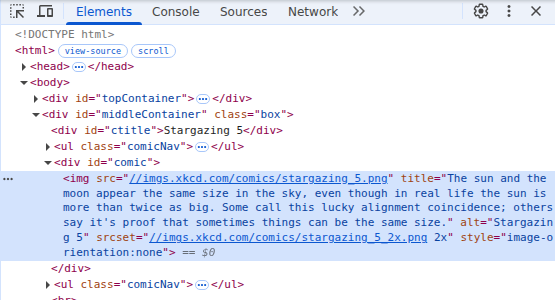
\includegraphics[width=\textwidth]{img/xkcd_inspect.png}
        \end{column}
    \end{columns}
\end{frame}

\begin{frame}[fragile]{Type, submit --- then wait \textit{well}}
    Fill a search box, submit, and wait for the exact condition instead of guessing a duration:
\begin{lstlisting}
from selenium.webdriver.common.keys import Keys
from selenium.webdriver.support.ui import WebDriverWait
from selenium.webdriver.support import expected_conditions as EC

driver.get("https://www.wikipedia.org")
box = driver.find_element(By.NAME, "search")
box.send_keys("Colorado Buffaloes")      # type like a user
box.send_keys(Keys.RETURN)               # submit the form

WebDriverWait(driver, 10).until(         # not a blind time.sleep(2)!
    EC.presence_of_element_located((By.ID, "firstHeading")))
print(driver.title)                      # -> Colorado Buffaloes - Wikipedia
\end{lstlisting}
    \texttt{WebDriverWait} polls every 0.5\,s, returns \textit{the instant} the condition holds, and raises \texttt{TimeoutException} if it never does --- faster, and it fails loudly. Common conditions: \texttt{presence\_of\_element\_located}, \texttt{visibility\_of\_element\_located}, \texttt{element\_to\_be\_clickable}.
\end{frame}

\begin{frame}[fragile]{Ten seconds of nothing}
    The same delayed page from Monday, in Selenium:
\begin{lstlisting}
driver.get("https://quotes.toscrape.com/js-delayed/")

element = WebDriverWait(driver, 15).until(          # 15 > the 10-second delay
    EC.presence_of_element_located((By.CLASS_NAME, "quote")))
print(len(driver.find_elements(By.CLASS_NAME, "quote")))   # 10
\end{lstlisting}
    A \texttt{time.sleep(2)} looks too early and finds nothing. \texttt{WebDriverWait} returns the moment the first quote appears --- about ten seconds here.

    \medskip
    Set the timeout longer than the slowest page you expect, and no longer than you can stand.
\end{frame}

\begin{frame}[fragile]{Scraping an infinite-scroll page}
    Scroll to the bottom, wait, and stop when the page stops growing:
\begin{lstlisting}
def scrape_infinite_scroll(driver, max_scrolls=20, pause=2):
    last = driver.execute_script("return document.body.scrollHeight")
    for i in range(max_scrolls):
        driver.execute_script("window.scrollTo(0, document.body.scrollHeight);")
        time.sleep(pause)                # let new content load
        new = driver.execute_script("return document.body.scrollHeight")
        if new == last:                  # height stopped growing -> the end
            break
        last = new
    return driver.page_source            # the fully-loaded HTML
\end{lstlisting}
    On \texttt{quotes.toscrape.com/scroll} it stops after ten scrolls with 100 quotes. Monday's Network tab check found the same 100 as JSON, with no browser.

    \medskip
    Set a sane \texttt{max\_scrolls}. \textbf{Proportionality} (Ch.~2): collect only what your question needs.
\end{frame}

\begin{frame}[fragile]{Selenium renders; BeautifulSoup reads}
    Get the page into the state you need, hand the rendered HTML to BeautifulSoup, and \textbf{always} clean up:
\begin{lstlisting}
from bs4 import BeautifulSoup

try:
    driver.get("https://quotes.toscrape.com/js/")
    WebDriverWait(driver, 10).until(
        EC.presence_of_element_located((By.CLASS_NAME, "quote")))
    soup = BeautifulSoup(driver.page_source, "html.parser")  # rendered HTML
    for item in soup.find_all("div", class_="quote"):
        text = item.find("span", class_="text")
        if text is None:             # same defensive habit as static scraping
            continue                 # skip a malformed item instead of crashing
        print(text.get_text(strip=True))
finally:
    driver.quit()                    # each driver is a whole browser process
\end{lstlisting}
    Selenium is the \textbf{hands} that navigate; BeautifulSoup is the \textbf{eyes} that read. \texttt{try/finally} guarantees the browser closes even when parsing throws.
\end{frame}

\begin{frame}{Three errors you will meet}
    \begin{columns}[T]
        \begin{column}{0.6\textwidth}
            \textbf{\texttt{NoSuchElementException}} --- the page has not finished loading. Wait on a condition.

            \medskip
            \textbf{\texttt{StaleElementReferenceException}} --- the page changed after you found the element. Find it again.

            \medskip
            \textbf{\texttt{SessionNotCreatedException}} --- the driver and the browser do not match. Remove the stray driver, or set \texttt{SE\_SKIP\_DRIVER\_IN\_PATH=true}.
        \end{column}
        \begin{column}{0.35\textwidth}
            \begin{alertblock}{Error flavors}
                \footnotesize Some failures \textit{are} the lesson (a page that is empty without JavaScript) --- that does not need a GitHub issue. Other code may be \textit{genuinely} broken: a selector a site renamed, a sandbox page that moved. Confirm it, then search and file an issue.
            \end{alertblock}
        \end{column}
    \end{columns}
\end{frame}

\begin{frame}{Lab: work these, then show-and-tell}
    \begin{columns}[T]
        \begin{column}{0.6\textwidth}
            Work in pairs. Do these exercises from the notebook:
            \begin{enumerate}\small
                \item Automate a search that has more than one step. Navigate to the page, enter the query, submit it, and extract the result.
                \item Examine three sites. Categorize each site as static, partially dynamic, or fully dynamic.
                \item Find a ``Load More'' button. Click it in a loop until it disappears. Count the items that were hidden.
                \item Measure the time for \texttt{requests}, for Selenium with a window, and for Selenium with no window. Report when the slower method is acceptable.
                \item Optional: rewrite your scraper as a Playwright script. Run it from a terminal.
                \item[6.] \textbf{5617}: use both methods on a research site that depends on JavaScript. Write a memo of about 500 words. Refer to \textcite{mitchell2018web}
            \end{enumerate}
        \end{column}
        \begin{column}{0.35\textwidth}
            \begin{block}{Submitting}
                \footnotesize Start in class, finish at home, submit what you got working.

                \smallskip

                Graded on good-faith attempt to complete rather than getting everything working.
            \end{block}
            \begin{block}{Show-and-Tell}
                \footnotesize Bring one of these to class: a bug you could not solve, data you find interesting, or a question for a research design.
            \end{block}
        \end{column}
    \end{columns}
\end{frame}

\begin{frame}[standout]
    The Twitter scraper that worked in 2019\\
    was dead by 2024.\\[1em]
    Browser automation is borrowed time ---\\
    {\large write it defensively, and expect it to break.}
\end{frame}

% =========================================================================
\section{Friday · Textbook Revisions}
% =========================================================================

\begin{frame}{Improving Chapter 8 together}
    \begin{columns}[T]
        \begin{column}{0.6\textwidth}
            Today we make the book better. Each of you opens a \textbf{pull request} against \texttt{ch-08-dynamic-pages.qmd} and reviews a classmate's.

            \bigskip

            The workflow (from Week 1):
            \begin{enumerate}\small
                \item Branch / fork the book repo
                \item Edit the chapter; commit with a clear message
                \item Open a PR describing \textit{what} and \textit{why}
                \item Review two peers' PRs: kind, specific, actionable
            \end{enumerate}

            \bigskip

            Review comments still follow Week 3's claim / link / sharpen taxonomy --- claim what you'll fix, link related issues, sharpen ones missing detail.
        \end{column}
        \begin{column}{0.35\textwidth}
            \centering
            
\includegraphics[width=\textwidth]{img/pr_review.png}
        \end{column}
    \end{columns}
\end{frame}

\begin{frame}{A revision menu for Chapter 8}
    High-value targets --- pick one and scope it to a single PR:
    \begin{itemize}
        \item \textbf{Test the code against live sites.} xkcd, Wikipedia, and the Quotes to Scrape sandbox all drift. Run the notebook headless, report what broke, and fix the selector --- the chapter's own ``Fragility Problem.''
        \item \textbf{Test the Playwright scripts.} Run the chapter's scripts from a terminal on your own machine. Report the download size and anything that differed on Windows or macOS.
        \item \textbf{Add the Firefox path.} Show Selenium Manager fetching \texttt{geckodriver}, and \texttt{playwright install firefox}, with what changed.
        \item \textbf{Try an agent on the sandbox.} Have an AI agent write a scraper for quotes.toscrape.com. Compare its script with yours, and add what you learned to ``Letting an AI Agent Drive.''
        \item \textbf{Strengthen an exercise.} Add expected output or a starter cell so an Additional Exercise is self-checking.
        \item \textbf{Extend ``Further Reading.''} A public-interest study that turned to browser automation after an API closed.
    \end{itemize}
\end{frame}

\begin{frame}{A good revision, and a good review}
    \begin{columns}[T]
        \begin{column}{0.6\textwidth}
            \begin{block}{A strong PR}
                \begin{itemize}\small
                    \item One focused change, clearly titled
                    \item Explains the problem it fixes
                    \item Builds (\texttt{quarto render}) without errors
                    \item Matches the book's voice and notation
                    \item Discloses any AI assistance
                \end{itemize}
            \end{block}
        \end{column}
        \begin{column}{0.35\textwidth}
            \begin{block}{A strong review}
                \begin{itemize}\small
                    \item Runs / reads the change, not just skims
                    \item Names specifics (line, claim, code)
                    \item Separates ``must fix'' from ``nice to have''
                    \item Is generous --- assume good faith
                    \item Ends with a clear verdict
                \end{itemize}
            \end{block}
        \end{column}
    \end{columns}
    \medskip
    \centering\small Next week: \textbf{Extracting data from PDFs} --- when the data isn't on a web page at all.
\end{frame}

% =========================================================================
\begin{frame}{Key takeaways}
    \begin{enumerate}
        \item Check by hand first: View Source, JavaScript off, the Network tab. The data is often already there.
        \item Selenium drives a \textbf{real browser} from your notebook. Selenium Manager fetches the driver, and the browser if you need one.
        \item Wait on \textbf{conditions}, not a blind \texttt{time.sleep()}. Render with a browser, read with BeautifulSoup, and \texttt{driver.quit()} every time.
        \item Playwright scripts the same work from a terminal. It waits on its own and records while you click.
        \item Agents can drive the browser, but for research, have them write a script you can rerun. \texttt{robots.txt} and ToS still apply.
    \end{enumerate}
    \bigskip
\end{frame}

\end{document}
